\chapter{O Dia da Semana com \texttt{scrdate}}
\begin{figure}[h]
    \centering
    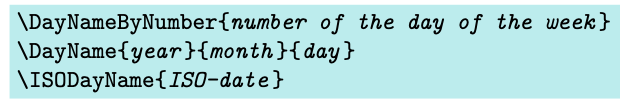
\includegraphics[width=0.75\linewidth]{imagem10.png}
\end{figure}

Normalmente, você está menos interessado no número do dia da semana do que em seu nome. Portanto, o comando \cmd{Day\-Na\-me\-By\-Num\-ber} retorna o nome do dia da semana correspondente a um número de dia da semana. Este número pode ser o resultado, por exemplo, de \cmd{Day\-Num\-ber} ou \cmd{ISO\-Day\-Num\-ber}. Os dois comandos \cmd{Day\-Na\-me} e \cmd{ISO\-Day\-Na\-me} retornam diretamente o nome do dia da semana de uma determinada data.

\bigskip
\textbf{Exemplo}: Você quer saber o nome do dia da semana de 24 de dezembro de 2027.

Por favor, pague por \cmd{ISODayName\{2027-12-24\}}, 24th~December~2027, a quantidade de\dots.  
\medskip

O resultado será:

Por favor, pague até sexta-feira, 24 de dezembro de 2027, o valor de\ldots

\medskip
Mais uma vez, vale a pena notar que você pode realizar cálculos, até certo ponto:

\bigskip
\textbf{Exemplo}: Você quer saber os nomes dos dias da semana 12 dias a partir de agora e 24 dias antes de 24 de dezembro de 2027.

\begin{figure}[h]
    \centering
    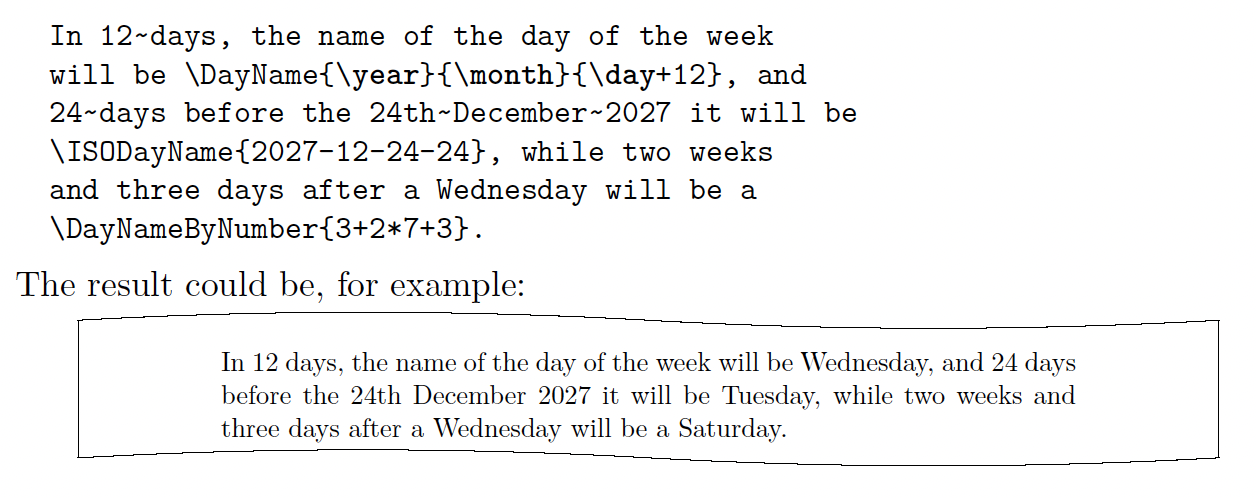
\includegraphics[width=0.9\linewidth]{imagem11.png}
\end{figure}

\begin{figure}[ht]
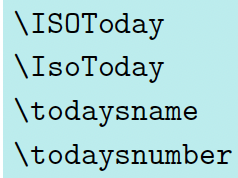
\includegraphics[width=0.25\linewidth]{imagem12.png}
\end{figure}
\newpage
Nos exemplos anteriores, a data atual sempre foi especificada de forma trabalhosa usando os registradores \TeX\ \cmd{year}, \cmd{month} e \cmd{day}. Os comandos \cmd{ISOToday} e \cmd{IsoToday} retornam diretamente a data atual em notação ISO. Esses comandos diferem apenas no fato de que \cmd{ISOToday} sempre gera um mês e dia de dois dígitos, enquanto \cmd{IsoToday} gera números de um único dígito para valores menores que 10. O comando \cmd{todays\-name} retorna diretamente o nome do atual dia da semana, enquanto \cmd{todays\-num\-ber} retorna o número do atual dia da semana. Você pode encontrar mais informações sobre o uso desse valor nas explicações de \cmd{Day\-Num\-ber} e \cmd{ISO\-Day\-Num\-ber}.

\begin{figure}[h]
    \centering
    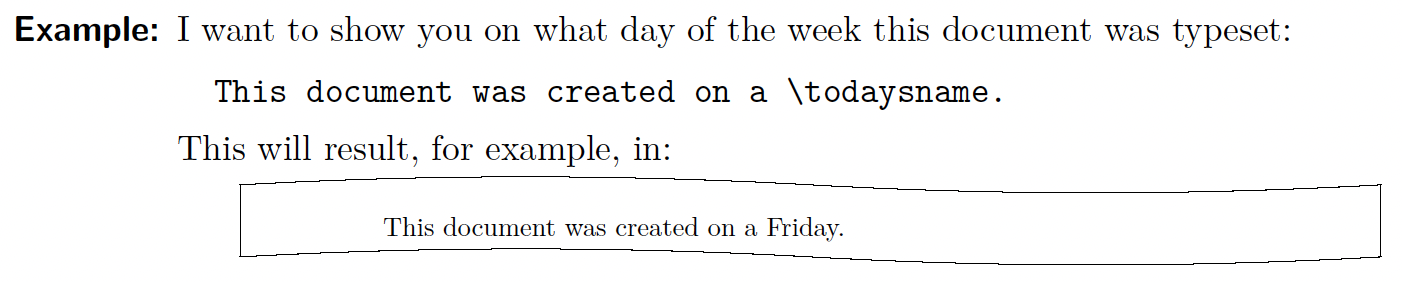
\includegraphics[width=1\linewidth]{imagem13.png}
\end{figure}

Para idiomas que têm um sistema de caso para substantivos, observe que o pacote não pode declinar palavras. Os termos são fornecidos na forma apropriada para exibir uma data em uma carta, que é o nominativo singular para os idiomas atualmente suportados. Dada essa limitação, o exemplo acima não funcionará corretamente se traduzido diretamente para alguns outros idiomas.

Os nomes dos dias da semana em \textbf{scrdate} têm letras iniciais maiúsculas. Se você precisar dos nomes completamente em letras minúsculas, por exemplo, porque essa é a convenção no idioma relevante, simplesmente envolva o comando com o comando \LaTeX\ \cmd{MakeLowercase}:

\verb|\MakeLowercase{\todaysname}|